
\documentclass[11pt,fleqn]{article} 
\usepackage[margin=0.8in, head=0.8in]{geometry} 
\usepackage{amsmath, amssymb, amsthm}
\usepackage{fancyhdr} 
\usepackage{palatino, url, multicol}
\usepackage{graphicx, pgfplots} 
\usepackage[all]{xy}
\usepackage{polynom} 
%\usepackage{pdfsync} %% I don't know why this messes up tabular column widths
\usepackage{enumerate}
\usepackage{framed}
\usepackage{setspace}
\usepackage{array,tikz}

\pgfplotsset{compat=1.6}

\pgfplotsset{soldot/.style={color=black,only marks,mark=*}} \pgfplotsset{holdot/.style={color=black,fill=white,only marks,mark=*}}


\pagestyle{fancy} 
\lfoot{}
\rfoot{FE Review Probs (day 1)}

\begin{document}
\renewcommand{\headrulewidth}{0pt}
\newcommand{\blank}[1]{\rule{#1}{0.75pt}}
\newcommand{\bc}{\begin{center}}
\newcommand{\ec}{\end{center}}
\renewcommand{\d}{\displaystyle}

\vspace*{-0.7in}

%%%%%%%%%intro page
\begin{center}
  \large
  \sc{Practice for the Final Exam (Day 2)}\\
  
\end{center}

\begin{enumerate}  
  \item  Find the Taylor series for the function $f(x) = \sin(x)$ centered at $a=\pi.$
\item  Use the integral test to determine whether $\d
    \sum_{n=1}^{\infty} n e^{-n^2} $ converges or diverges. 
    \item Determine whether the series $\d \sum_{n=1}^{\infty} (-1)^n \frac{\sqrt n}{2n +3}$ is absolutely convergent, conditionally convergent  or
  divergent. You must clearly explain your reasoning. 
\item Find the radius of convergence and the interval of convergence
  of the following series. 

  \begin{enumerate}
  \item $\d \sum_{n=1}^{\infty} n! ( 2x - 1)^n$
  \item $\d \sum_{n=1}^{\infty} \frac{(x-a)^n}{n b^n}$, where $a$ and
    $b$ are positive constants.
  \end{enumerate}



\item Consider $x = t^2 + 1$, $y = e^{2t} - 1$. 
  \begin{enumerate}
  \item Find $\d \frac{dy}{dx}$.
  \item Determine the location of any horizontal tangents. If none
    exist, explain why. 
  \item Find $\d \frac{d^2 y}{dx^2}$.
  \item Determine the concavity of the graph when $t=1.$
  \vfill
  \end{enumerate}
\item Consider the curve $r = 1 + 2 \cos \theta$. 
  \begin{enumerate}
  \item Sketch the curve $r = 1 + 2 \cos \theta$. Include the coordinates of all $x$- and $y$-intercepts.\\
  
  
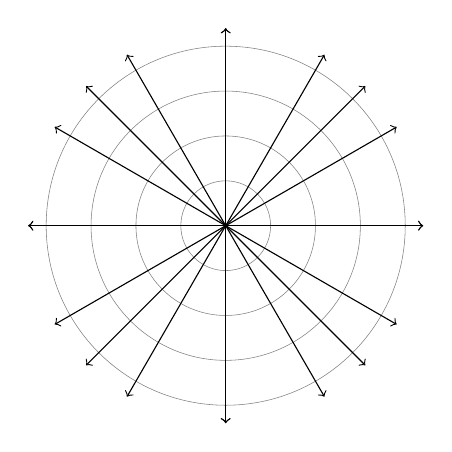
\begin{tikzpicture}[scale=0.57,baseline=(current bounding
        box.center)]
        \foreach \i in {1,2,3,4}{ \draw[help lines] (0,0) circle (\i)
          ; }

        %\foreach{\i} in {1,2,3,4}{ \draw (\i, 0) node[below
          %right]{\i}; \draw (0,\i) node[above right] {\i}; }

        \foreach \i in {30, 60, ..., 360} \draw[->] (0,0) -- (\i:4.4);

        \foreach \i in {45, 90, ..., 360} \draw[->] (0,0) -- (\i:4.4);
      \end{tikzpicture}


  \item Set up an integral to find the area enclosed by the inner loop. (You should be able to evaluate it but you can think about that later.)
 
  \end{enumerate}
  
  \item  For each problem below, set up an integral(s) to find the quantity.
  	\begin{enumerate}
	\item Find the mass of a wire that is 2 meters long (starting at $x=0$) and has density $\rho(x)=3x+1$ grams per meter.
	\item Let $\mathcal{R}$ be the region bounded by $y = e^x$ and $y =
  0$, $0 \le x \le 2$. If the density of the region is given by $\rho=5,$ find the center of mass of $R$ (or, equivalently, find the centroid of $R.$)
  	\item Recall that in the metric system force, $F$, is often measured in newtons ($N$) and work, $W$, is often measured in joules ($j$) or newton-meters ($N\cdot m$). Suppose a spring has a natural length of $15$ cm and exerts a force of $8$ N when stretched to a length of 20 cm. How much work is done stretching the spring from $15$ cm to $25$ cm?
    	\end{enumerate}
 \end{enumerate}
\end{document}

